% !TEX root = ../my_thesis.tex
\pagebreak
\section{Stand der Forschung und Grundlagen}

Dieses Kapitel versucht einen Überblick des Forschungsstandes in den unterschiedlichen Aspekten der Arbeit zu verschaffen. Anschließend vermittelt das Kapitel notwendige Grundkenntnisse.

\subsection{Einführung}


% SLAM, visual Odometrie, Viewpoint,

% Lokalisierungsproblem erläutern
% Ansätze aufzählen
% Überführen auf visuelle Lokalisierung
// Evt. Einblick über indoor Lokalizierungstechnicken \\

\textbf{Pose Estimation} wird in dieser Arbeit als eine Methode der visuellen Lokalisierung (\textit{Visual-Based Localization, kurz VBL}) betrachtet. VBL beschäftigt sich mit der Bestimmung der Pose (\textit{Position + Orientierung}) eines visuellen Abfragematerials (\textit{z.B. ein RGB-Bild}) in einer zuvor bekannten Szene  \cite{piascoSurveyVisualBasedLocalization2018}.
Ein naheliegendes Themengebiet der Robotik ist die visuelle Ortswiedererkennung (\textit{Visual Place Recognition, kurz VPR}) \cite{lowryVisualPlaceRecognition2016}. Die visuelle Ortswiedererkennung fokussiert sich auf das Feststellen eines bereits besuchten Ortes und definiert sich aus einer Mapping-, Datenverarbeitungs- und einem Orientierungsmodul. Allgemein lässt sich das Prozess eines VPRs folgend beschreiben. Eine interne Karte bekannter Orte wird durch das Mappingmodul verwaltet. Die Daten werden vom Datenverarbeitungsmodul vorbereitet und anschließend an das Orientierungsmodul übergeben. Daraufhin bestimmt das Orientierungsmodul die Pose und entscheidet mit der immer aktuell gehaltenen Karte, ob ein Ort bereits besucht wurde.  Im Vergleich zur VPR versucht die visuelle Lokalisierung eine Pose zu bestimmen und benötigt daher neben den zwei Modulen kein Mappingmodul.

% hat 2 katogiren..
Die rein visuellen Methoden des VBLs unterteilen sich in indirekte und direkte Methoden \cite{lowryVisualPlaceRecognition2016}. Die indirekten Methoden behandeln das Lokalisierungsproblem als eine Bildersuche in einer Datenbank, ähnlich wie das \textit{Content Based Image Retrieval} \cite{lewContentbasedMultimediaInformation2006} Problem. Dabei wird das Abfragebild über eine Ähnlichkeitsfunktion mit den Vergleichsbildern aus der Datenbank abgeglichen \cite{zhangImageBasedLocalization2006, arandjelovicThreeThingsEveryone2012, radenovicCNNImageRetrieval2016}. Diese Art von Methoden benötigen eine sehr große Bildergalerie (\textit{Datenbank}) und liefern Ergebnisse bei Fund eines korrespondierenden Bildes \cite{lowryVisualPlaceRecognition2016}. Hingen versuchen die direkten Methoden die Pose über eine Referenzumgebung zu bestimmen und benötigen meist daher keine große Bildergalerie  \cite{piascoSurveyVisualBasedLocalization2018}. Es gibt drei Arten der direkten Methoden: 
\begin{enumerate*}[label=\arabic*)]
	\item Abgleichen von Features zu Punktwolken (\textit{z.B. \cite{liWorldwidePoseEstimation2012}})
	\item Pose Regression mit Tiefenbilder (\textit{z.B. \cite{shottonSceneCoordinateRegression2013a}})
	\item Pose Regression nur mit Bildern (\textit{z.B. \cite{kendallPoseNetConvolutionalNetwork2015}})
\end{enumerate*}

Die erste Art von Methoden versucht die Pose zu bestimmen, indem die 2D-3D Korrespondenz über das Abgleichen von Features des Abfragebildes gegen die Deskriptoren der 3D-Punkte hergestellt werden \cite{irscharaStructurefrommotionPointClouds2009, liWorldwidePoseEstimation2012, svarmCityScaleLocalizationCameras2017}. Diese Vorgehensweise hat Ähnlichkeiten zu den indirekten Methoden und benötigt statt einer Bildergalerie eine repräsentative 3D-Punktwolke der Szene \cite{piascoSurveyVisualBasedLocalization2018}. Die zweite Art von Methoden bestimmt anhand von Tiefenbilder die Pose z.B. über Regression Forests \cite{shottonSceneCoordinateRegression2013a}, Randomize Ferns \cite{glockerRealTimeRGBDCamera2015}, Coarse-to-Fine Registierung \cite{santosMappingIndoorSpaces2016} oder Neuronale Netze \cite{massicetiRandomForestsNeural2016}. Diese Forschungsprojekte liefern mit 3D-Bildern gewünschte Resultate. Die Ergebnisse sind abhängig von 3D-Kameras, diese sind jedoch nicht verbreitet.

\textbf{Convolutional Neural Networks} (\textit{CNN}) werden erfolgreich im Bereich des Maschinelles Sehens, wie z.B. bei der Klassifizierung von Bildern \cite{krizhevskyImageNetClassificationDeep2012, simonyanVeryDeepConvolutional2014, heDeepResidualLearning2015} sowie bei der Objekterkennung \cite{girshickRichFeatureHierarchies2013, renFasterRCNNRealTime2015b, girshickFastRCNN2015} eingesetzt. 
Ein verbreiteter Ansatz beim Entwurf von CNNs ist das häufig zweckentfremdende Feintunen (\textit{fine-tune}) der Netzwerkarchitekturen, die z.B. für die Bildklassifizierung angesichts der Aufgaben von ImageNet \cite{russakovskyImageNetLargeScale2014} konstruiert wurden. Dieser Ansatz konnte beispielsweise erfolgreich in der Objekterkennung \cite{girshickFastRCNN2015}, Objektsegmentierung \cite{kokkinosPushingBoundariesBoundary2015, maninisConvolutionalOrientedBoundaries2016}, semantische Segmentierung \cite{nohLearningDeconvolutionNetwork2015, hazirbasFuseNetIncorporatingDepth2017a} und Tiefenbestimmung \cite{liDepthSurfaceNormal2015} verfolgt werden.
Seit Kurzem werden CNNs auch in den Anwendungsgebieten der Lokalisierung verwendet. Zum Beispiel verwenden  \citet{parisottoGlobalPoseEstimation2018} CNNs in Bezug auf das Simultaneous-Localization-and-Mapping (\textit{SLAM}) Problem. \citet{melekhovRelativeCameraPose2017} schätzen anhand CNNs die relative Pose zweier Kameras. \citet{costanteExploringRepresentationLearning2016} und \citet{wangDeepVOEndtoendVisual2017} setzen es im Bereich der visuellen Odometrie ein.

% Posenet überführen & erklären
Geleitet von den \textit{state-of-the-art} Lokalisierungsergebnissen der CNNs stellen \citet{kendallPoseNetConvolutionalNetwork2015} den ersten Ansatz zu direkten Posebestimmung nur mit RGB-Bildern vor. PoseNet ist die Modifikation der GoogLeNet \cite{szegedyGoingDeeperConvolutions2015} Architektur und zweckentfremdet es von der Bildklassifizierung zu einem Pose-Regressor. Trainiert mit einem Datensatz, bestehend aus Paaren von Farbbild und Pose, kann es die sechs Freiheitsgrade der Kamerapose in unbekannten Szenen mittels eines Bildes bestimmen. Dieser Ansatz benötigt weder eine durchsuchbare Bildgalerie noch eine Punktwolke oder Tiefenbilder der Szene. Im Vergleich zu den metrischen Ansätzen wie SLAM oder visuelle Odometrie liefert es eine weniger akkurate Pose. Es bietet jedoch eine hohe Toleranz gegenüber Skalierungs- und Erscheinungsänderungen des Anfragebildes an \cite{piascoSurveyVisualBasedLocalization2018}.

% Varianten aufzählen
Es gibt mehrere Ansätze, die die Genauigkeit von PoseNet übertreffen.
Einen Fortschritt erhalten die Autoren von PoseNet durch die hier \cite{kendallModellingUncertaintyDeep2015a} vorgestellte Anpassung ihres Models an einem Bayessian Neural Network \cite{denkerTransformingNeuralNetOutput1991, mackayPracticalBayesianFramework1991}.
Dieselben Autoren erweitern PoseNet mit einer neuen Kostenfunktion unter Berücksichtigung von geometrischen Eigenschaften \cite{kendallGeometricLossFunctions2017}. \citet{walchImagebasedLocalizationUsing2016} und \citet{clarkVidLocDeepSpatioTemporal2017} setzen Long-Short-Term-Memory (\textit{LSTM}) \cite{hochreiterLongShortTermMemory1997a} Einheiten ein, um Wissen aus der Korrelation von Bildsequenzen zu gewinnen. \citet{wuDelvingDeeperConvolutional2017} und \citet{naseerDeepRegressionMonocular2017} augmentieren den Trainingsdatensatz. \citet{wuDelvingDeeperConvolutional2017} stocken den vorhandenen Datensatz auf, indem sie die Bilder künstlich rotieren. \citet{naseerDeepRegressionMonocular2017} erweitern zuerst über ein weiteres CNN den Datensatz um Tiefenbildern. Anschließend simulieren die Autoren RGB-Bilder aus verschiedenen Viewpoints. Im Vergleich zu PoseNet verwenden \citet{mullerSQUEEZEPOSENETIMAGEBASED2017} und \citet{melekhovImageBasedLocalizationUsing2017} eine andere Architektur. 
Das Modell von \citet{mullerSQUEEZEPOSENETIMAGEBASED2017} basiert auf die SqueezeNet \cite{iandolaSqueezeNetAlexNetlevelAccuracy2016} Architektur. \citet{melekhovImageBasedLocalizationUsing2017} stellen HourglassNet, basierend auf einem symmetrischen Encoder-Decoder Architektur, vor. \citet{brahmbhattGeometryAwareLearningMaps2018} und \citet{valadaDeepAuxiliaryLearning2018, valadaIncorporatingSemanticGeometric} binden zusätzliche Informationen wie z.B. visuelle Odometrie, GPS oder IMU ein. 

Jedes dieser Ansätze benötigen annotierte Traininsdaten. Für die Erstellung solcher Daten wurden beispielsweise mit entsprechender Hardware ausgerüstete Trolleys \cite{huitlTUMindoorExtensiveImage2012}, 3D-Kameras \cite{izadiKinectFusionRealtime3D2011} oder SfM-Methoden \cite{kendallPoseNetConvolutionalNetwork2015} eingesetzt.

% Simulierte 3D-Daten 
\textbf{Simulierte 3D-Daten} werden in der Literatur oft eingesetzt, um das manuelle Erzeugen und Annotieren von Daten umzugehen. \citet{pishchulinArticulatedPeopleDetection2012a}, \citet{pengLearningDeepObject2014}, \citet{suRenderCNNViewpoint2015} und \citet{varolLearningSyntheticHumans2017} erzeugen ihren Trainingsdaten, indem sie virtuelle Objekte auf reale Hintergrundbildern platzieren. \citet{pishchulinArticulatedPeopleDetection2012a} generieren Daten zwecks Personenerkennung und Bestimmung derer körperlicher Pose. Zuvor werden auf den vorhandenen Bildern die körperliche Pose der Personen bestimmt und daran deren 3D Modelle rekonstruiert. Anschließend werden die 3D-Modelle in ihrer Pose variiert auf reale Hintergrundbildern platziert. \citet{pengLearningDeepObject2014} erstellen Daten, um Objekte auf realen Bildern zu detektieren. Von jeder Objektklasse werden 3D-Modelle auf einem Hintergrundbild aus einer Sammlung gelegt. \citet{suRenderCNNViewpoint2015} generieren einen großen Datensatz mit 3D-Modellen, um den Viewpoint von Objekten auf realen Bildern zu bestimmen. Bei dieser Datengenerierung wird jedes virtuelle Objekt auf zufällige Hintergrundbildern positioniert und mit unterschiedlichen Konfigurationen (\textit{z.B. Beleuchtung}) gerendert. \citet{varolLearningSyntheticHumans2017} erstellen künstliche Personen auf Bildern, um beispielsweise den menschlichen Körper in seine Glieder zu segmentieren. Dabei rendern sie zufällige virtuelle Personen mit zufälliger Pose auf beliebige Hintergrundbildern. \citet{fanelloLearningBeDepth2014} rendert künstliche Infrarotbilder von Händen sowie Gesichtern zwecks Tiefenerkennung und Segmentierung der Hand in den einzelnen Fingern sowie des Gesichtes in Bereiche aus einem RGB-Bild. \citet{dosovitskiyFlowNetLearningOptical2015} erlernen mit synthetischen Daten den optischen Fluss von Bildsequenzen.  Hierbei werden auf Hintergrundbildern aus einer Sammlung mehrmals bewegte virtuelle Stühle platziert.

Motiviert von der Datengenerierung über 3D-simulierten Daten stellt \citet{haImagebasedIndoorLocalization2018} einen Ansatz zur Bild-basierte Lokalisierung in Gebäuden vor. Dieser Forschungsansatz generiert synthetische Daten aus einem Building-Information-Modeling (\textit{BIM}). Bei den Daten werden die durch das vortrainierte VGG Netzwerk \cite{simonyanVeryDeepConvolutional2014} extrahierte Features als wesentlich erachtet und in einer Datenbank gepflegt. Ein reales Aufnahmebild im Gebäude lässt sich durch den Vergleich der Features lokalisieren. \citet{acharyaBIMPoseNetIndoorCamera2019, acharyaMODELLINGUNCERTAINTYSINGLE2019} erzeugen ebenso Trainingsdaten aus einem BIM, jedoch verwenden sie zur Lokalisierung keine Datenbank bedürftiges Verfahren, sondern bestimmen die Pose direkt über PoseNet. Die Daten werden entlang einer Flugbahn aus der Simulation eines Korridors gesammelt. Hierbei werden sich in der Realitätstreue vom karikaturistisch zu fotorealistisch hin über zu fotorealistisch-texturiert unterscheidende Daten erzeugt. Die besten Ergebnisse konnten die Autoren trainiert mit den Gradienten- und Kantenbilder der karikaturistischen Daten, getestet auf die Gradientenbilder der realen Aufnahmen, erzielen.
\\\\// Anbindung zu meinem Beitrag
\\\\
Im weiteren Verlauf des Kapitels werden einige grundlegende Themen erläutert. Zuerst werden künstliche neuronale Netze definiert. Danach wird ein vertieftes Wissen an CNN vermittelt und anschließend bekannte CNN Modelle näher erläutert.

%\subsection{Lineare Faltung}
%\subsubsection{Sobelfilter}
%\subsubsection{Gradientenbild}
%Bei der Erzeugung von Gradienten- bzw. Kantenbilder gehen einerseits wichtige Informationen im Hinblick auf das Ursprungsbild verloren, andererseits bleiben wichtige Informationen wie z.B. die geometrische Struktur erhalten.

\subsection{Künstliche neuronale Netzwerke}
Inspiriert von ihren biologischen Vorbildern \footnote{das Nervensystem eines Lebewesen, z.B. des Menschen}, vernetzen künstliche neuronale Netzwerke (\textit{KNN}) künstliche Neuronen miteinander.

Ein einzelnes Neuron erhält einen Inputsignal auf mehreren Kanälen und löst erst ein Signal (\textit{output}) aus, falls die gewichtete Summe des Inputs einen gewissen Schwellwert erreicht \cite{CS231nConvolutionalNeural}. Abbildung \ref{fig:neuron} stellt eine beispielhafte Visualisierung eines künstlichen Neurons dar.

Sei $x$ das Input, $w$ der Gewichtsvektor, $b$ ein Bias, $f$ eine nicht-lineare \textit{Aktivierungsfunktion}, dann ist ein künstliches Neuron mit der Inputsgröße $I$ mathematisch eine nicht-lineare Funktion $\textbf{n} : \mathbb{R}^I \mapsto \mathbb{R}$ \cite{CS231nConvolutionalNeural}:
\begin{equation}
	\label{eq:neuron}
	\quad	\textbf{n(x)}=f\left(\sum_i w_{i} x_{i} + b\right) = f(W^Tx+b)
\end{equation}


\begin{figure}
	\centering
	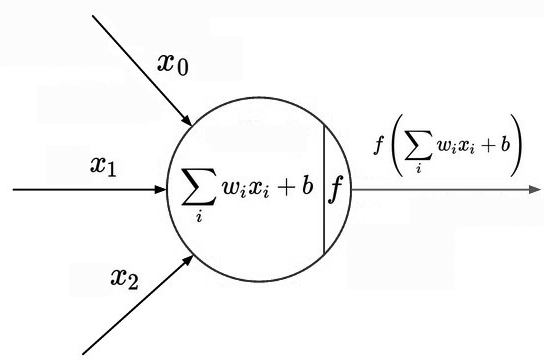
\includegraphics[width=0.5\textwidth]{images/neuron_model.png}
	\caption{Visualisierung eines künstlichen Neurons definiert nach der Gleichung \ref{eq:neuron}. Dieser Neuron summiert das Produkt des Inputvektors $x = (x_0, x_1, x_2)$  mit den jeweiligen Gewichten und addiert einen Bias $b$. Durch die Summe erzeugt die Aktivierungsfunktion $f$ das Output des Neurons. Entnommen aus \cite{CS231nConvolutionalNeural}}
	\label{fig:neuron}
\end{figure}

Künstliche Neuronen können zu einer Schicht (\textit{layer}) zusammengeführt werden. Mehrere solcher Schichten bilden einen Netzwerk. Bei einem \textit{feedforward} Netzwerk übergibt jedes Neuron aus der Schicht $l$ seinen Output an die Neuronen des Schichtes $l+1$ weiter \cite{Goodfellow-et-al-2016}. Diese Einschränkung gilt nicht bei \textit{feedback} Netzwerken, auch bekannt als \textit{Recurrent Neural Networks}\footnote{Recurrent Neural Networks werden in dieser Arbeit nicht mehr behandelt}.


Die Tiefe (\textit{depth}) eines Netzwerks wird dabei durch die Anzahl der Schichten bestimmt\footnote{der Input-Schicht ist ausgeschloßen} und die Breite (\textit{width}) eines Schichtes wird durch die Anzahl der Neuronen  bestimmt\cite{Goodfellow-et-al-2016}.

\begin{figure}
	\centering
	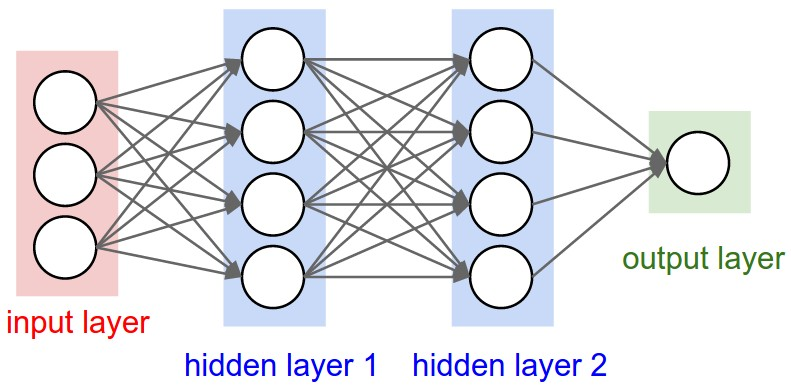
\includegraphics[width=0.7\textwidth]{images/neural_net.jpeg}
	\caption{Ein \textit{feedforwad} neuronales Netz mit der Tiefe 3 bestehend aus einem Input der Breite 3, aus zwei \textit{Hidden-Layer }der Breite 4 und einem \textit{Output-Layer} der Breite 1.  Entnommen aus \cite{CS231nConvolutionalNeural}}
	\label{fig:neural_net}
\end{figure}

Das Netz lernt durch die Anpassung der Gewichte.
\subsection{Convulutional Neural Networks}
\subsubsection{Convolution Layer}
\subsubsection{Pooling Layer}
\subsubsection{Fully Connected Layer}
\subsection{Bekannte CNN Modelle}
\subsubsection{GoogLeNet}
\subsubsection{PoseNet}

\pagebreak